\documentclass[12pt]{article}
\usepackage{marktext} 
%% Remove draft for real article, put twocolumn for two columns
\usepackage{svmacro}
\usepackage[utf8]{inputenc}
\usepackage[style=alphabetic, backend=biber]{biblatex}
\addbibresource{bibliography.bib}
\newcommand{\vect}{\mathbf}

%% commentary bubble
\newcommand{\SV}[2][]{\sidenote[colback=green!10]{\textbf{SV\xspace #1:} #2}}

%% Title 
\title{ MATH 104: Multivariable Calculus}
%\author[1]{Co-author}
\author{Name: \_ \_ \_ \_ \_ \_ \_ \_ \_ \_ \_ \_ \_ \_ \_ \_ \_}
%\affil[1]{Institute}
\date{\today}

\begin{document}

\maketitle

\section*{Rules}

\begin{itemize}
    \item 5 questions, 90 minutes
    \item Closed books
    \item Show all your work. Mere numbers for solutions will not count for grades.
    \item No sharing of calculators
\end{itemize}

\section*{Scores}

\begin{enumerate}[Problem 1.]
    \item  \_\_\_/20
    \item  \_\_\_/20
    \item \_\_\_/20
    \item  \_\_\_/20
    \item  \_\_\_/20
\end{enumerate}
Total \_\_\_\_\_\_\_\_/100


\newpage
\section*{Questions}

\begin{problem}Let $f:\R^2 \to \R$.
    \begin{enumerate}[a.]
        \item  What does it mean for $f$ to be 
            differentiable at $(a,b)$?
        \item What does it mean for $f$ to have a directional derivative
            in the direction of $\textbf{u}$? What's a notation for this notion?
        \item Write directional derivative of function $f$ in the direction $\textbf{u}$ in terms of partial derivative/gradient of $f$.
        \item Let $f:\R^2 \to \R$ be a function and $C$ be a smooth curve in $\R^2$ parametrized by $\vect{r}:[a,b]\to \R^2$. Write down the formula to compute the line integral of $f$ over $C$.
    \end{enumerate}
\end{problem}


\newpage
\begin{problem}
    \begin{enumerate}[a.]
        \item Consider the vector field
            \begin{equation*}
                \vect{F}(x,y) = x^2 \vect{j} \,.
            \end{equation*}
            Is the integral $\int_C \vect{F} \cdot d\vect{r}$ independent of path?

        \item 
            Compare
            the path integrals of $\vect{F}$ on two paths $A\to B \to C$ and $A\to D \to C$,
            where the paths are from the figure below.
            \begin{figure}[!h]
            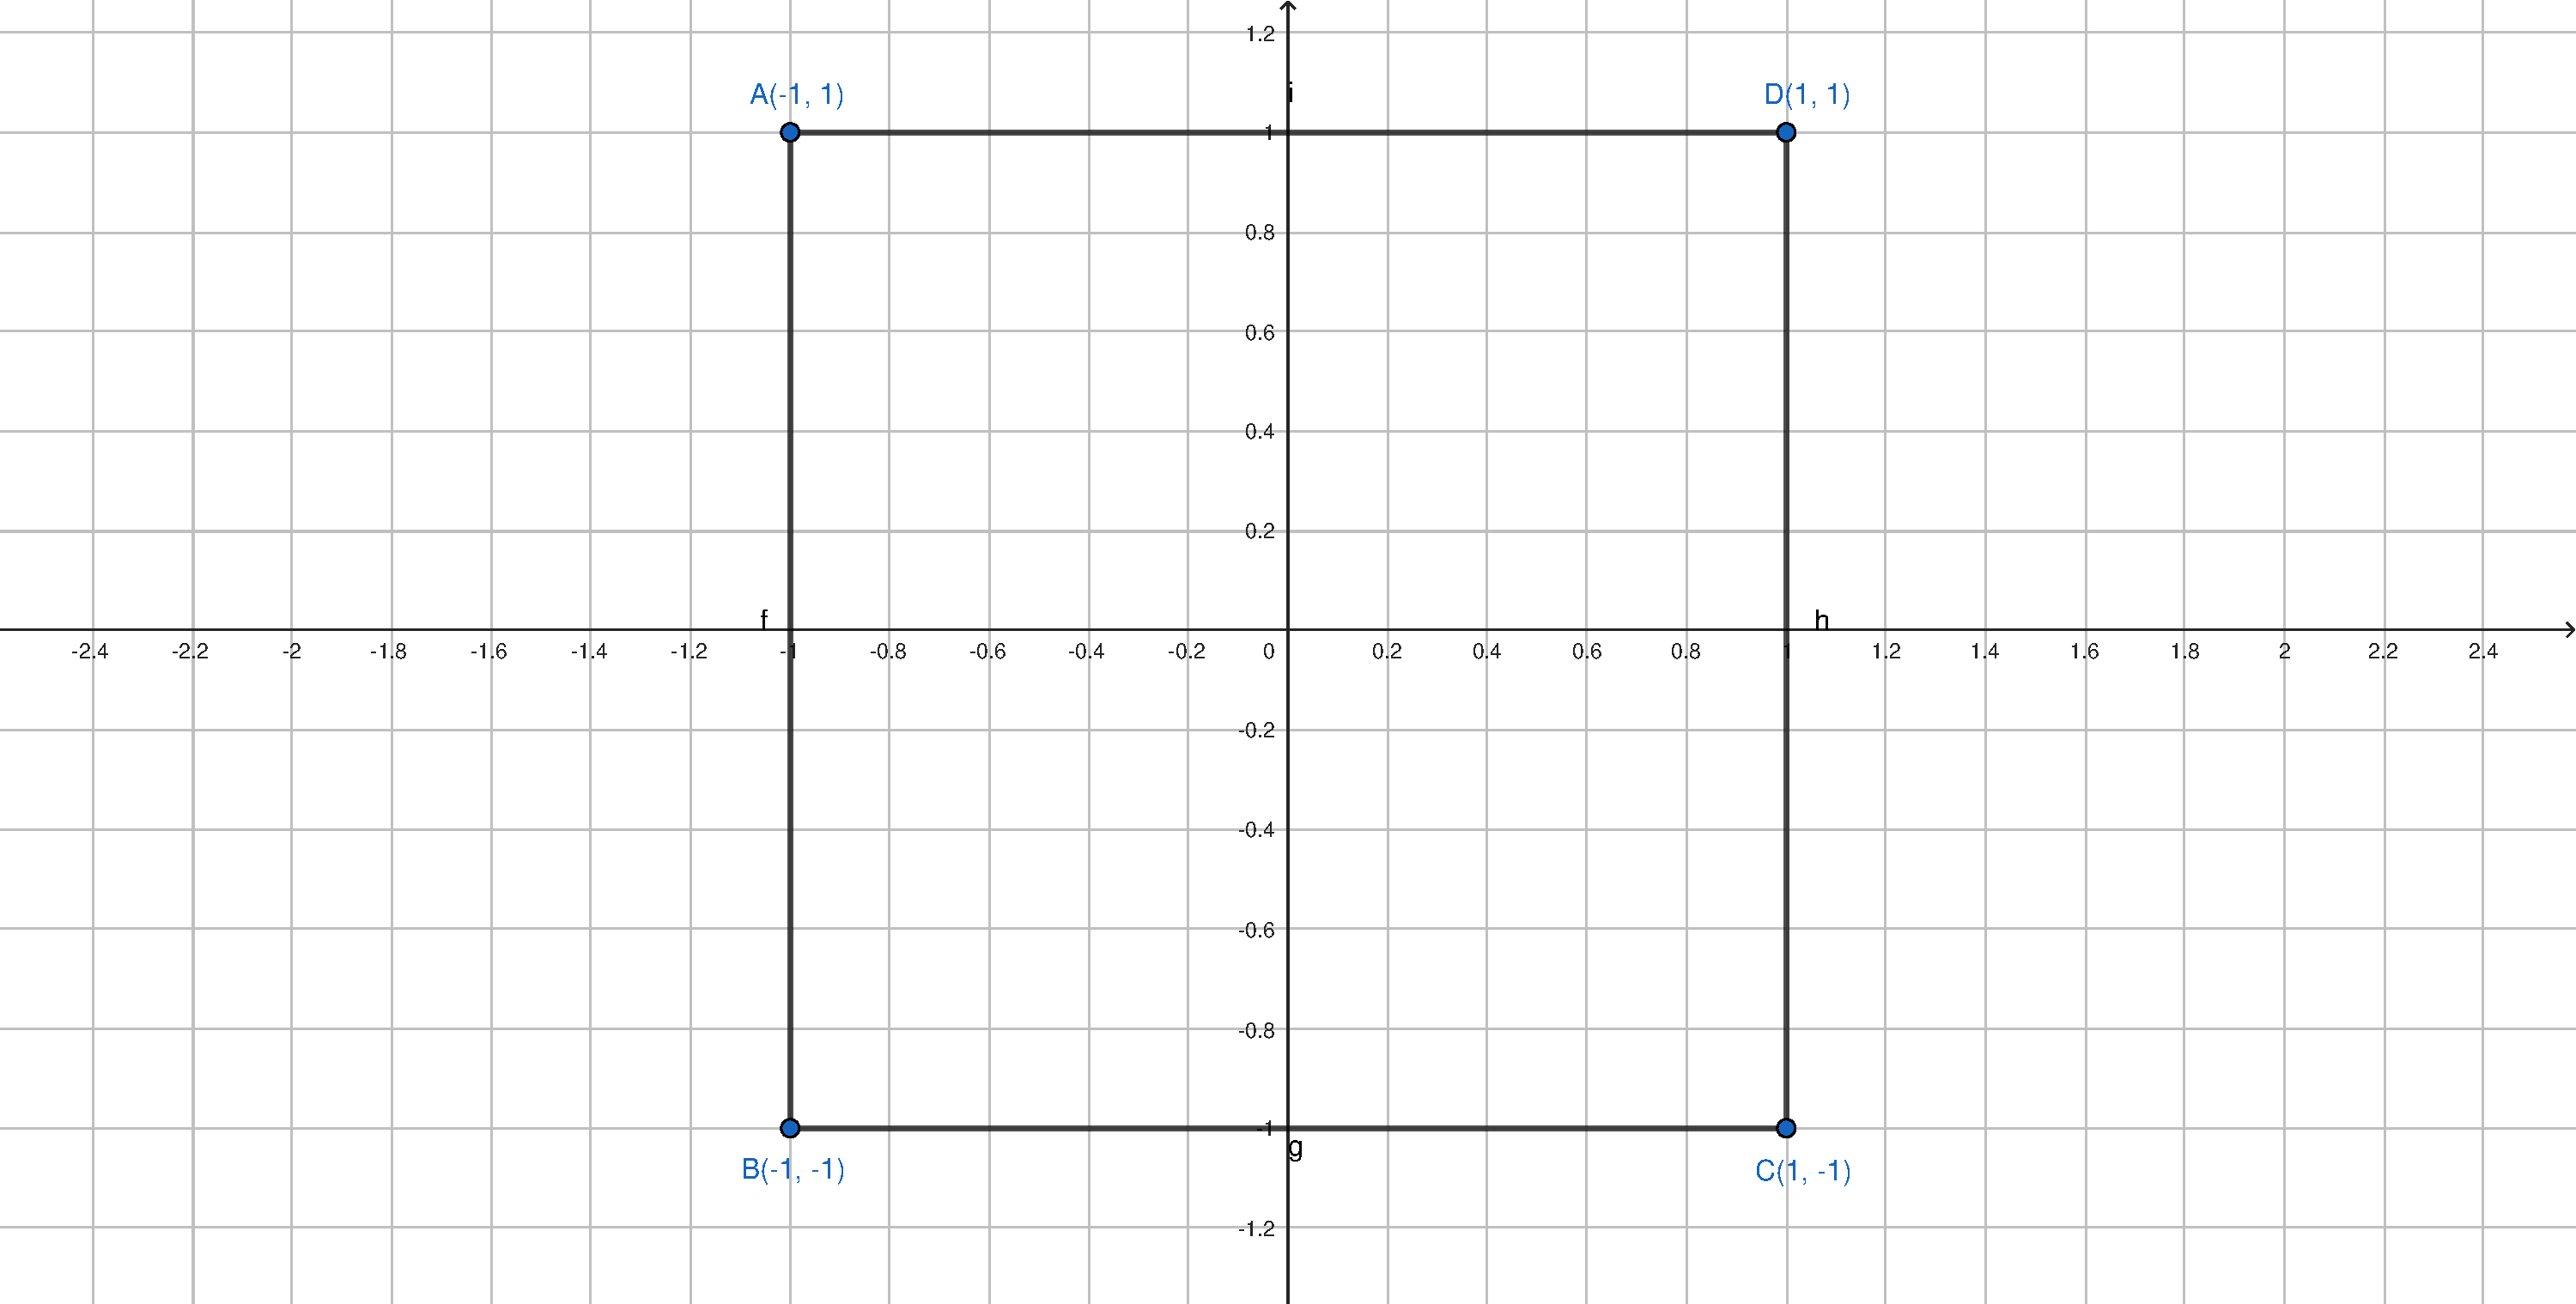
\includegraphics[width=1.5\textwidth]{paths.pdf}
            \end{figure}
    \item Are parts (a) and (b) consistent with each other? Why or why not?
    \end{enumerate}

\end{problem}


\newpage
\begin{problem}
\begin{enumerate}
    \item Given a function $f:\R^n \to \R$, where $n\geq 2$.
        What are the properties of $\grad f$? (List everything that you can think of)
    \item Given any surface $F(x,y,z) = C$, where $F$ is differentiable everywhere, how do you know there's only one tangent plane at a given point?
        (Give the best answer you can)
    \item Find the tangent plane to the surface
        \begin{equation*}
            x^2 + 2xy - y^2 + z^2 =7 
        \end{equation*}
        at point
        \begin{equation*}
            P_0(1,-1,3) \,.
        \end{equation*}
\end{enumerate}
\end{problem}


\newpage
\begin{problem}
    \begin{enumerate}
        \item Find the tangent vector, normal vector and curvature of the following curve
    \begin{equation*}
        \textbf{r}(t) = \langle \cos t + t \sin t, \sin t - t\cos t, 3 \rangle \,.
    \end{equation*}
    \item What's the meaning of the curvature of a curve at a point on the curve?
    \end{enumerate}

\end{problem}

\newpage

\begin{problem}
    \begin{enumerate}
        \item State the second derivative test when you want to optimize a differentiable function $f:\R^2 \to \R$.
        \item Find all the local maxima, local minima, and saddle points (neither min nor max) of the function
    \begin{equation*}
        f(x,y) = \ln(x+y) + x^2 - y \,.
    \end{equation*}
    \end{enumerate}
\end{problem}
%\bibliography{refs}


\end{document}
